% Options for packages loaded elsewhere
\PassOptionsToPackage{unicode}{hyperref}
\PassOptionsToPackage{hyphens}{url}
%
\documentclass[
  12pt,
]{article}
\usepackage{amsmath,amssymb}
\usepackage{lmodern}
\usepackage{setspace}
\usepackage{iftex}
\ifPDFTeX
  \usepackage[T1]{fontenc}
  \usepackage[utf8]{inputenc}
  \usepackage{textcomp} % provide euro and other symbols
\else % if luatex or xetex
  \usepackage{unicode-math}
  \defaultfontfeatures{Scale=MatchLowercase}
  \defaultfontfeatures[\rmfamily]{Ligatures=TeX,Scale=1}
\fi
% Use upquote if available, for straight quotes in verbatim environments
\IfFileExists{upquote.sty}{\usepackage{upquote}}{}
\IfFileExists{microtype.sty}{% use microtype if available
  \usepackage[]{microtype}
  \UseMicrotypeSet[protrusion]{basicmath} % disable protrusion for tt fonts
}{}
\makeatletter
\@ifundefined{KOMAClassName}{% if non-KOMA class
  \IfFileExists{parskip.sty}{%
    \usepackage{parskip}
  }{% else
    \setlength{\parindent}{0pt}
    \setlength{\parskip}{6pt plus 2pt minus 1pt}}
}{% if KOMA class
  \KOMAoptions{parskip=half}}
\makeatother
\usepackage{xcolor}
\usepackage[margin=1in]{geometry}
\usepackage{graphicx}
\makeatletter
\def\maxwidth{\ifdim\Gin@nat@width>\linewidth\linewidth\else\Gin@nat@width\fi}
\def\maxheight{\ifdim\Gin@nat@height>\textheight\textheight\else\Gin@nat@height\fi}
\makeatother
% Scale images if necessary, so that they will not overflow the page
% margins by default, and it is still possible to overwrite the defaults
% using explicit options in \includegraphics[width, height, ...]{}
\setkeys{Gin}{width=\maxwidth,height=\maxheight,keepaspectratio}
% Set default figure placement to htbp
\makeatletter
\def\fps@figure{htbp}
\makeatother
\setlength{\emergencystretch}{3em} % prevent overfull lines
\providecommand{\tightlist}{%
  \setlength{\itemsep}{0pt}\setlength{\parskip}{0pt}}
\setcounter{secnumdepth}{-\maxdimen} % remove section numbering
\usepackage{amssymb}
\usepackage{amsmath}
\usepackage{subfig}
\usepackage{booktabs}
\usepackage{longtable}
\usepackage{array}
\usepackage{multirow}
\usepackage{wrapfig}
\usepackage{float}
\usepackage{colortbl}
\usepackage{pdflscape}
\usepackage{tabu}
\usepackage{threeparttable}
\usepackage{threeparttablex}
\usepackage[normalem]{ulem}
\usepackage{makecell}
\usepackage{xcolor}
\ifLuaTeX
  \usepackage{selnolig}  % disable illegal ligatures
\fi
\IfFileExists{bookmark.sty}{\usepackage{bookmark}}{\usepackage{hyperref}}
\IfFileExists{xurl.sty}{\usepackage{xurl}}{} % add URL line breaks if available
\urlstyle{same} % disable monospaced font for URLs
\hypersetup{
  pdftitle={Econ771 - Empirical Exercise 1},
  pdfauthor={Nixon Torres Candiales},
  hidelinks,
  pdfcreator={LaTeX via pandoc}}

\title{Econ771 - Empirical Exercise 1}
\author{Nixon Torres Candiales}
\date{\today}

\begin{document}
\maketitle

\setstretch{1.25}
\hypertarget{summary-statistics}{%
\section{Summary Statistics}\label{summary-statistics}}

Provide and discuss a table of simple summary statistics showing the
mean, standard deviation, min, and max of hospital total revenues and
uncompensated care over time. We start first by downloading and merging
all the Data from the Github repository. We present the distribution of
the variables of interest, Uncompensated care and Hospital Revenue over
time

\begin{figure}
\subfloat[Uncompensated Care\label{fig:Fig-1-1}]{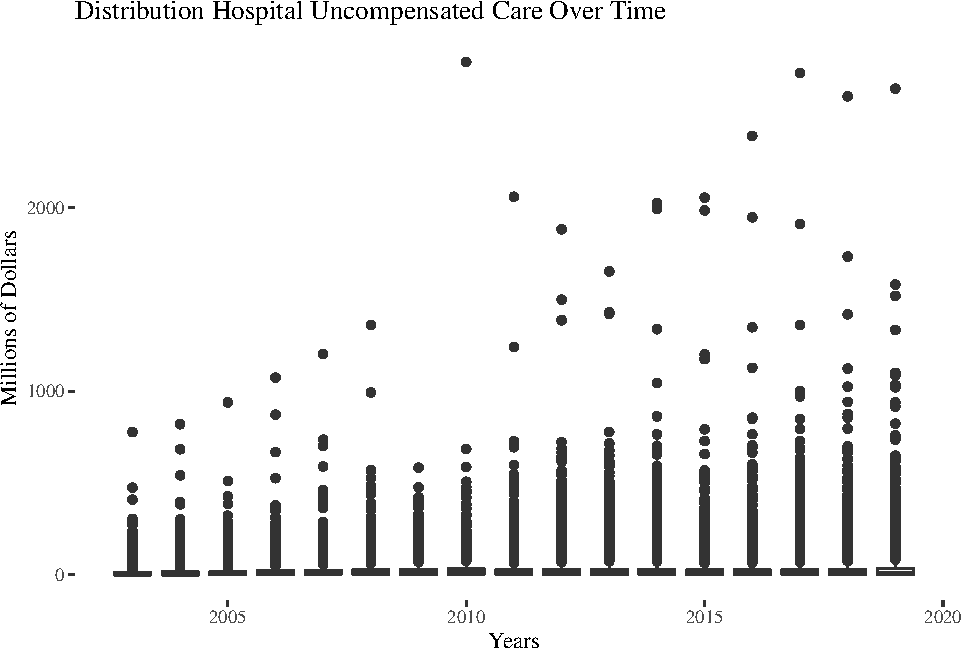
\includegraphics[width=.49\linewidth]{Report_files/figure-latex/Fig-1-1} }\subfloat[Revenue\label{fig:Fig-1-2}]{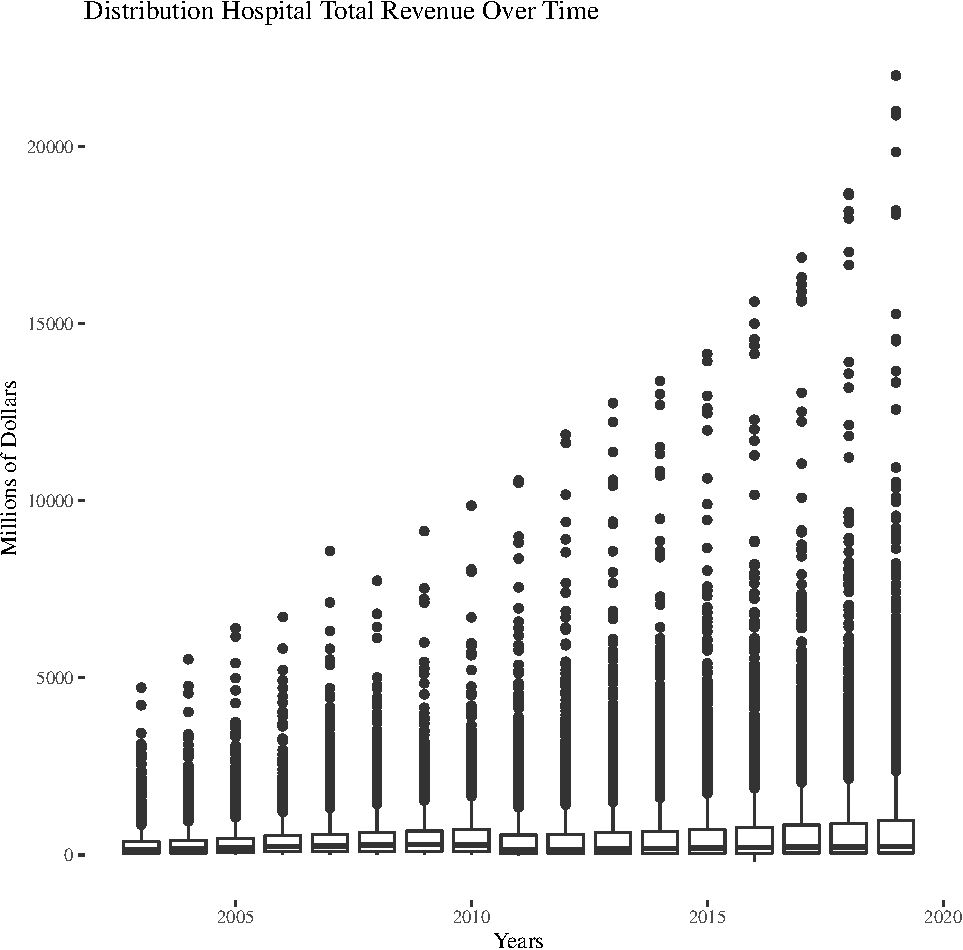
\includegraphics[width=.49\linewidth]{Report_files/figure-latex/Fig-1-2} }\caption{Box-plot}\label{fig:Fig-1}
\end{figure}

We see evidence of negative entries in uncompensated care as well as
extreme atypical values that might be caused by mistyping. As such, we
subset the data by not including the top and bottom 0.5\% of the
observations. The mean, standard deviation, and minimum and maximum
values across the years are presented in table 1 of summary statistics.

\begin{longtable}[t]{crrrrrrrr}
\caption{\label{tab:Tab-1}Hospital Summary Statistics}\\
\toprule
\multicolumn{1}{c}{ } & \multicolumn{4}{c}{Uncompensated Care} & \multicolumn{4}{c}{Total Revenue} \\
\cmidrule(l{3pt}r{3pt}){2-5} \cmidrule(l{3pt}r{3pt}){6-9}
year & Mean & Sd & Min & Max & Mean & Sd & Min & Max\\
\midrule
2003 & 13.25 & 30.67 & -0.13 & 777.99 & 284.34 & 383.67 & 1.66 & 4722.76\\
2004 & 15.16 & 37.51 & 0.00 & 820.25 & 316.73 & 430.15 & 0.27 & 5525.73\\
2005 & 17.31 & 39.89 & 0.00 & 939.13 & 364.92 & 495.20 & 1.14 & 6398.55\\
2006 & 20.52 & 49.08 & -2.67 & 1074.62 & 415.62 & 540.55 & 1.33 & 6718.17\\
2007 & 22.85 & 52.29 & 0.00 & 1203.37 & 462.17 & 622.69 & 0.99 & 8577.05\\
\addlinespace
2008 & 25.81 & 58.58 & 0.00 & 1361.81 & 492.36 & 634.20 & 0.97 & 7743.08\\
2009 & 26.51 & 44.88 & 0.00 & 583.98 & 527.15 & 687.54 & 0.89 & 9139.32\\
2010 & 28.59 & 67.33 & 0.00 & 2793.92 & 548.93 & 749.12 & 0.84 & 9857.53\\
2011 & 25.12 & 59.19 & -54.28 & 2059.70 & 450.38 & 743.80 & -27.58 & 10572.29\\
2012 & 27.95 & 67.66 & -7.44 & 1882.62 & 473.44 & 795.60 & 0.85 & 11865.32\\
\addlinespace
2013 & 30.15 & 68.89 & -4.50 & 1652.58 & 507.13 & 868.88 & 0.95 & 12751.71\\
2014 & 30.30 & 73.99 & -25.85 & 2024.85 & 544.82 & 949.87 & 1.09 & 13376.35\\
2015 & 28.58 & 71.70 & -0.03 & 2054.15 & 588.68 & 1013.22 & 1.05 & 14143.53\\
2016 & 36.60 & 379.86 & -0.02 & 20405.51 & 640.63 & 1118.53 & -177.03 & 15618.75\\
2017 & 32.07 & 84.51 & -0.03 & 2733.60 & 689.32 & 1220.53 & 1.00 & 16863.43\\
\addlinespace
2018 & 34.70 & 88.22 & -0.06 & 2606.35 & 742.95 & 1341.00 & 1.07 & 18677.25\\
2019 & 38.55 & 97.95 & -97.31 & 2648.26 & 814.30 & 1488.31 & 0.72 & 22000.93\\
2003-2019 & 28.17 & 123.62 & -97.31 & 20405.51 & 546.30 & 960.02 & -177.03 & 22000.93\\
\bottomrule
\end{longtable}

Next, we create a figure showing the mean hospital uncompensated care
from 2003 to 2019. We show this trend separately by hospital ownership
type in figure 3. We present an smooth trend to easily identify shifts
after the adoption of medicare expansion in 2014. We can see an abrupt
bump from years 2010 to 2011, this might be due to the adoption of the
new form and a change in the way to measure uncompensated care
\^{}{[}after 2010 uncompensated care = total uncompensated care - total
uncompensated partial payments + bad debt{]}. Also, in recent years, it
seems for-profit hospitals get to provide more uncompensated care than
not for profit hospitals.

\begin{figure}
\centering
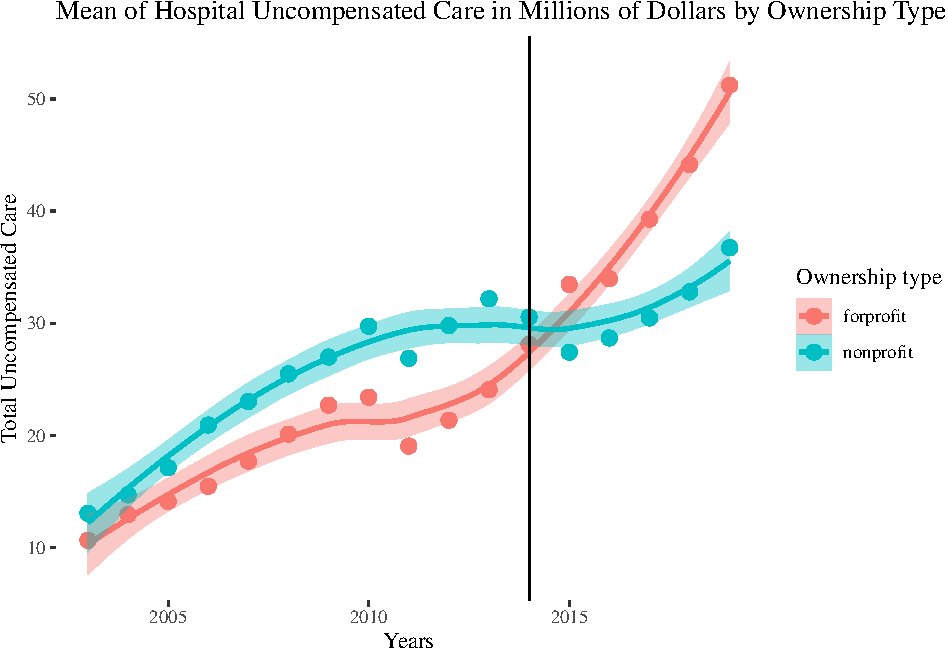
\includegraphics{Report_files/figure-latex/Fig-2-1.pdf}
\caption{Evolution of Uncompensated Care Over Time}
\end{figure}

\newpage

\hypertarget{twfe-specification}{%
\section{TWFE Specification}\label{twfe-specification}}

Using a simple DD identification strategy, we estimate the effect of
Medicaid expansion on hospital uncompensated care using a traditional
two-way fixed effects (TWFE) estimation:

\begin{equation}
\label{eq:dd}
y_{it} = \alpha_{i} + \gamma_{t} + \delta D_{it} + \varepsilon_{it},
\end{equation}

where \(D_{it}=1(E_{i}\leq t)\) in Equation \ref{eq:dd} is an indicator
set to 1 when a hospital is in a state that expanded as of year \(t\) or
earlier, \(\gamma_{t}\) denotes time fixed effects, \(\alpha_{i}\)
denotes hospital fixed effects, and \(y_{it}\) denotes the hospital's
amount of uncompensated care in year \(t\). We present four estimates
from this estimation in table \ref{Tab-2}: one based on the full sample
(1); one when limiting to the 2014 treatment group (2); one when
limiting to the 2015 treatment group (3); and one when limiting to the
2016 treatment group (3).

A first appreciation of our results indicate that the ATE of medicaid
expansion on uncompensated care is negative. The point estimate varies
when limiting the treatment sample for 2014 to 2016 as well as the
confidence intervals but we get a consistent trend across the samples.
We see the effect is larger when limiting the sample to the states that
expanded in 2014.

\begin{table}

\caption{\label{tab:Tab-2}Two Way Fixed Effects}
\centering
\begin{tabular}[t]{lcccc}
\toprule
\multicolumn{1}{c}{ } & \multicolumn{4}{c}{Uncompensated Care} \\
\cmidrule(l{3pt}r{3pt}){2-5}
  & Full Sample & 2014 Sample & 2015 Sample & 2016 Sample\\
\midrule
Treatment & -29.325*** & -32.655*** & -29.471*** & -28.495***\\
 & (1.903) & (2.198) & (2.721) & (2.056)\\
\midrule
Num.Obs. & 61856 & 54268 & 31112 & 29201\\
R2 & 0.701 & 0.712 & 0.700 & 0.712\\
RMSE & 39.37 & 39.88 & 49.07 & 48.52\\
Std.Errors & by: pn & by: pn & by: pn & by: pn\\
\bottomrule
\multicolumn{5}{l}{\rule{0pt}{1em}+ p $<$ 0.1, * p $<$ 0.05, ** p $<$ 0.01, *** p $<$ 0.001}\\
\end{tabular}
\end{table}

\newpage

\hypertarget{event-study-specification}{%
\section{Event Study Specification}\label{event-study-specification}}

We estimate an event study version of the specification in part 3:

\begin{equation}
\label{eq:event}
y_{it} = \alpha_{i} + \gamma_{t} +\sum_{\tau < -1} D_{it}^{\tau} \delta_{\tau} + \sum_{\tau>=0} D_{it}^{\tau} \delta_{\tau} + \varepsilon_{it},
\end{equation}

where \(D_{it}^{\tau} = 1(t-E_{i}=\tau)\) in Equation \ref{eq:event} is
an interaction between the treatment indicator and a relative time
indicator. \(\tau\) denotes years relative to Medicaid expansion. In
this case \(\tau=-1\) denotes the year before a state expanded Medicaid
and the control group for those never treated. \(\tau=0\) denotes the
year of expansion, and so on.

Table \ref{Tab-3} presents the estimates for the common treatment time
for the 2014 sample, whereas \ref{Tab-4} presents the estimates for the
staggered intervention for the full sample. In both specifications the
control group is formed by the never treated. Also, we can observe in
\ref{Fig-2} the event study coefficients plot. It is clear the drop in
uncompensated care after the first year of the medicaid expansion. Also
the ATT seems to increase as \(\tau\) increases. We can see that the
average treatment on the treated is the highest 5 years after the
treatment.

\begin{table}

\caption{\label{tab:Tab-3}Event Study}
\centering
\begin{tabular}[t]{lcc}
\toprule
\multicolumn{1}{c}{ } & \multicolumn{2}{c}{Uncompensated Care} \\
\cmidrule(l{3pt}r{3pt}){2-3}
  & 2014 Sample & Full Sample\\
\midrule
relative\_time = -11 × treated & 12.035*** & 16.239***\\
 & (2.957) & (3.226)\\
relative\_time = -10 × treated & 12.513*** & 13.289***\\
 & (2.634) & (2.593)\\
relative\_time = -9 × treated & 14.104*** & 13.266***\\
 & (2.780) & (2.619)\\
relative\_time = -8 × treated & 15.928*** & 14.152***\\
 & (3.303) & (2.764)\\
relative\_time = -7 × treated & 15.397*** & 13.013***\\
 & (3.377) & (2.751)\\
relative\_time = -6 × treated & 12.872*** & 11.425***\\
 & (3.373) & (2.643)\\
relative\_time = -5 × treated & 9.445*** & 10.264***\\
 & (2.851) & (3.040)\\
relative\_time = -4 × treated & 7.515** & 4.279*\\
 & (2.608) & (1.896)\\
relative\_time = -3 × treated & 3.080** & 3.600***\\
 & (1.122) & (0.893)\\
relative\_time = -2 × treated & 0.495 & 1.317*\\
 & (0.880) & (0.557)\\
relative\_time = 0 × treated & -11.639*** & -10.221***\\
 & (0.941) & (0.651)\\
relative\_time = 1 × treated & -21.077*** & -20.028***\\
 & (1.315) & (1.054)\\
relative\_time = 2 × treated & -24.200*** & -24.963***\\
 & (1.436) & (1.304)\\
relative\_time = 3 × treated & -29.086*** & -29.634***\\
 & (1.676) & (1.525)\\
relative\_time = 4 × treated & -32.339*** & -32.660***\\
 & (1.793) & (1.714)\\
relative\_time = 5 × treated & -37.156*** & -37.071***\\
 & (2.088) & (2.024)\\
\midrule
Num.Obs. & 54268 & 61856\\
RMSE & 39.73 & 39.18\\
Std.Errors & by: pn & by: pn\\
FE: pn & X & X\\
FE: year & X & X\\
\bottomrule
\multicolumn{3}{l}{\rule{0pt}{1em}+ p $<$ 0.1, * p $<$ 0.05, ** p $<$ 0.01, *** p $<$ 0.001}\\
\end{tabular}
\end{table}

\begin{figure}
\centering
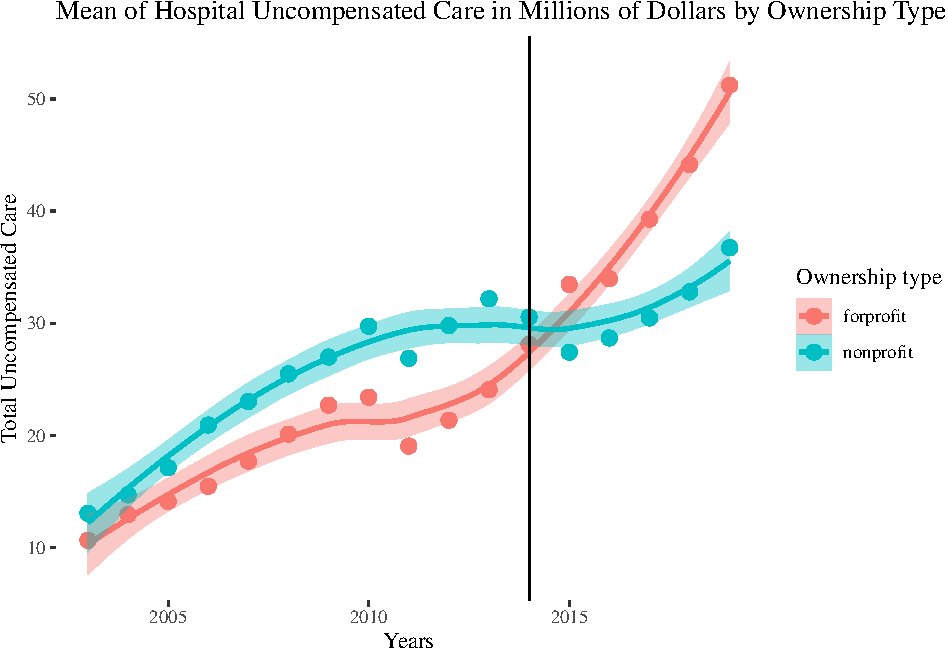
\includegraphics{Report_files/figure-latex/Fig-3-1.pdf}
\caption{Event Study}
\end{figure}

\newpage

\hypertarget{sa-specification}{%
\section{SA Specification}\label{sa-specification}}

No we move to Sun and Abraham(SA) specification and estimate a
non-conxvex average of all other group-time specific average treatment
effects. The interaction weighted specification is given by:

\begin{equation}\label{eq:iwevent}
y_{it} = \alpha_{i} + \gamma_{t} +\sum_{e} \sum_{\tau \neq -1} \left(D_{it}^{\tau} \times 1(E_{i}=e)\right) \delta_{e, \tau} + \varepsilon_{it}.
\end{equation}

\ref{table-5} presents the Re-estimate coefficients for the event study
using the SA specification. For this specification we focus on the
states that expanded either on 2014, 2015 or 2016 and include those in
the treatment group. Whereas the control group is formed by the never
treated observations. Providers that are in a state that expanded after
2016 are not considered in this part. The coefficients presented in the
table are \(\hat{\delta}_{e, \tau}\).

\begin{table}

\caption{\label{tab:Tab-4}Event Estudy Sun and Abraham(SA) Specification}
\centering
\begin{tabular}[t]{lccc}
\toprule
\multicolumn{1}{c}{ } & \multicolumn{3}{c}{Uncompensated Care} \\
\cmidrule(l{3pt}r{3pt}){2-4}
  & 2014 Sample & 2015 Sample & 2016 Sample\\
\midrule
time\_to\_treat = -7 & 14.282*** & -0.704 & -8.627+\\
 & (2.696) & (3.178) & (5.167)\\
time\_to\_treat = -6 & 12.448*** & -3.045 & -12.580***\\
 & (2.856) & (2.335) & (3.619)\\
time\_to\_treat = -5 & 10.754*** & 2.300 & -8.890**\\
 & (2.867) & (5.836) & (2.767)\\
time\_to\_treat = -4 & 6.472** & -5.025*** & -8.697***\\
 & (1.966) & (1.367) & (2.257)\\
time\_to\_treat = -3 & 3.650*** & -3.000*** & -6.676***\\
 & (0.992) & (0.884) & (1.354)\\
time\_to\_treat = -2 & 1.337+ & -1.956** & -4.002***\\
 & (0.697) & (0.696) & (0.914)\\
time\_to\_treat = 0 & -10.782*** & -4.164*** & -6.574***\\
 & (0.766) & (0.878) & (0.731)\\
time\_to\_treat = 1 & -19.683*** & -7.731*** & -12.905***\\
 & (1.140) & (1.046) & (1.789)\\
time\_to\_treat = 2 & -23.433*** & -11.979*** & -16.813***\\
 & (1.300) & (1.181) & (1.886)\\
time\_to\_treat = 3 & -28.423*** & -15.415*** & -21.161***\\
 & (1.543) & (1.256) & (2.023)\\
time\_to\_treat = 4 & -31.627*** & -13.092*** & \\
 & (1.735) & (1.574) & \\
time\_to\_treat = 5 & -37.157*** &  & \\
 & (2.089) &  & \\
\midrule
Num.Obs. & 61856 & 61856 & 61856\\
RMSE & 39.16 & 39.92 & 39.96\\
Std.Errors & by: pn & by: pn & by: pn\\
FE: pn & X & X & X\\
FE: year & X & X & X\\
\bottomrule
\multicolumn{4}{l}{\rule{0pt}{1em}+ p $<$ 0.1, * p $<$ 0.05, ** p $<$ 0.01, *** p $<$ 0.001}\\
\end{tabular}
\end{table}

Also, \Ref{Fig-5} presents the coefficients plot for the SA
specification. We can see how this smooth the pre-trend before the
medicaid expansion. Under this especification we see the Uncompensated
care is significatly declining even before the expansion.

\begin{figure}
\centering
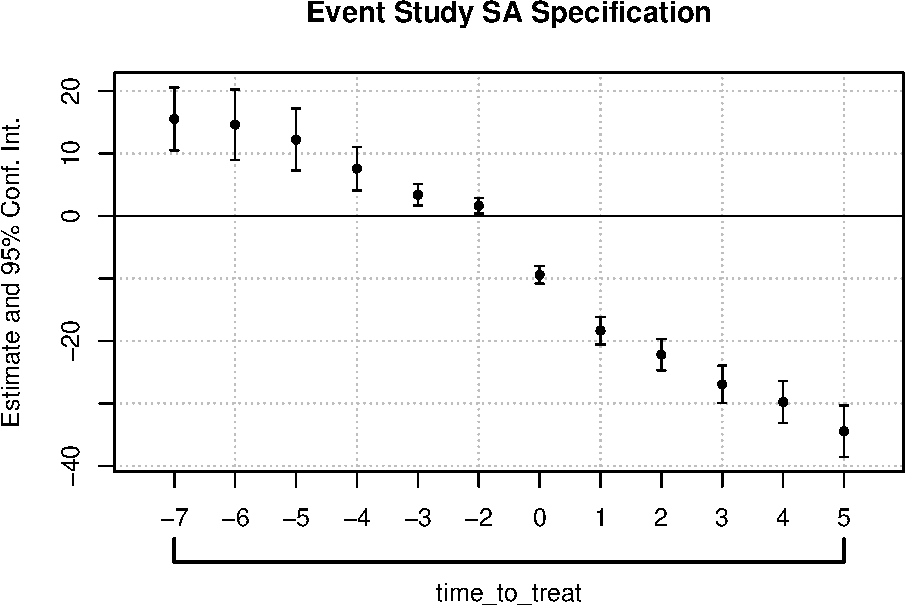
\includegraphics{Report_files/figure-latex/Fig-4-1.pdf}
\caption{Effect of Medicaid Eaxpansion on Uncompensated Care - SA
Specification for different treatment samples}
\end{figure}

\newpage

\hypertarget{cs-specification}{%
\section{CS Specification}\label{cs-specification}}

Callaway and Sant'Anna (CS) offer a non-parametric solution that
effectively calculates a set of group-time specific differences,
\(ATT(g,t)= E[y_{it}(g) - y_{it}(\infty) | G_{i}=g]\), where \(g\)
reflects treatment timing and \(t\) denotes time. They show that under
the standard DD assumptions of parallel trends and no anticipation,
\(ATT(g,t) = E[y_{it} - y_{i, g-1} | G_{i}=g] - E[y_{it} - y_{i,g-1} | G_{i} = \infty]\),
so that \(\hat{ATT}(g,t)\) is directly estimable from sample analogs. CS
also propose aggregations of \(\hat{ATT}(g,t)\) to form an overall ATT
or a time-specific ATT (e.g., ATTs for \(\tau\) periods before/after
treatment). With this framework in mind, provide an alternative event
study using the CS estimator. Hint: check out the \texttt{did} package
in \texttt{R} or the \texttt{csdid} package in \texttt{Stata}.

\begin{figure}
\subfloat[ATT by Cohorts\label{fig:Fig-5-1}]{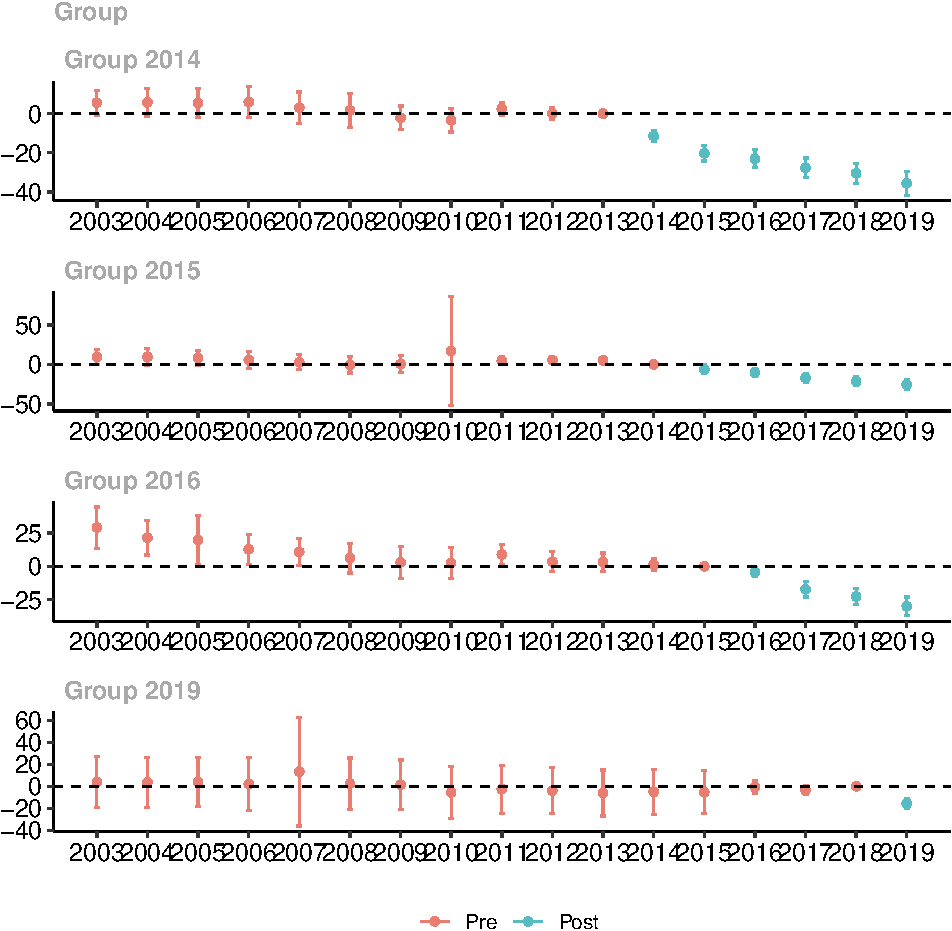
\includegraphics[width=.49\linewidth]{Report_files/figure-latex/Fig-5-1} }\subfloat[Event Study\label{fig:Fig-5-2}]{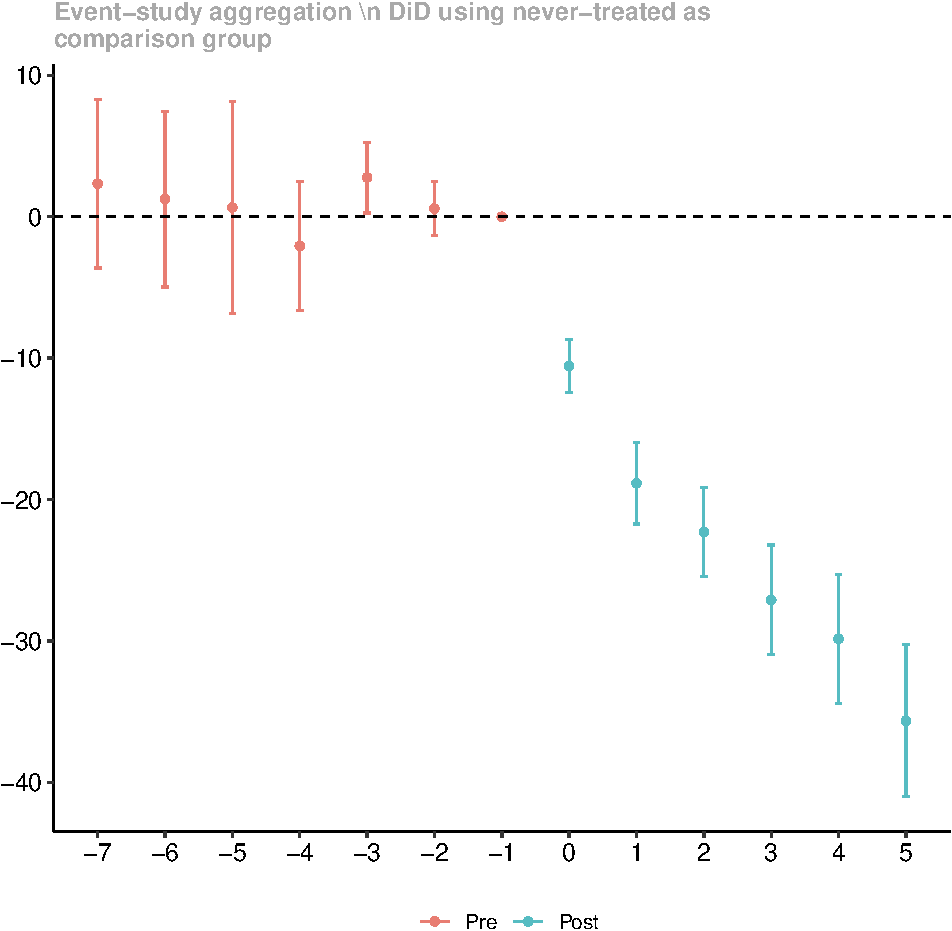
\includegraphics[width=.49\linewidth]{Report_files/figure-latex/Fig-5-2} }\caption{Callaway and Sant’Anna (CS) Specification}\label{fig:Fig-5}
\end{figure}

\begin{table}

\caption{\label{tab:Tab-6}DiD CS Specification}
\centering
\fontsize{6}{8}\selectfont
\begin{tabular}[t]{lc}
\toprule
\multicolumn{1}{c}{ } & \multicolumn{1}{c}{ATT(g,t)} \\
\cmidrule(l{3pt}r{3pt}){2-2}
  & Est.\\
\midrule
ATT(2014,2003) & 5.619 [-0.700, 11.939]\\
ATT(2014,2004) & 5.711 [-1.447, 12.869]\\
ATT(2014,2005) & 5.374 [-1.977, 12.724]\\
ATT(2014,2006) & 5.922 [-2.024, 13.867]\\
ATT(2014,2007) & 3.030 [-4.969, 11.028]\\
ATT(2014,2008) & 1.638 [-6.995, 10.272]\\
ATT(2014,2009) & -2.067 [-8.013, 3.879]\\
ATT(2014,2010) & -3.365 [-9.433, 2.703]\\
ATT(2014,2011) & 2.530 [-0.804, 5.864]\\
ATT(2014,2012) & 0.090 [-2.867, 3.047]\\
ATT(2014,2013) & 0.000\\
ATT(2014,2014) & -11.446 [-14.307, -8.585]\\
ATT(2014,2015) & -20.250 [-24.223, -16.276]\\
ATT(2014,2016) & -23.016 [-27.708, -18.324]\\
ATT(2014,2017) & -27.688 [-32.717, -22.659]\\
ATT(2014,2018) & -30.492 [-35.599, -25.384]\\
ATT(2014,2019) & -35.639 [-41.762, -29.516]\\
ATT(2015,2003) & 9.581 [0.270, 18.891]\\
ATT(2015,2004) & 9.444 [-0.880, 19.768]\\
ATT(2015,2005) & 8.175 [-1.766, 18.117]\\
ATT(2015,2006) & 5.645 [-4.887, 16.176]\\
ATT(2015,2007) & 2.815 [-6.803, 12.432]\\
ATT(2015,2008) & -0.399 [-10.735, 9.938]\\
ATT(2015,2009) & 0.605 [-9.691, 10.901]\\
ATT(2015,2010) & 16.846 [-51.909, 85.600]\\
ATT(2015,2011) & 4.925 [-0.451, 10.301]\\
ATT(2015,2012) & 5.675 [1.859, 9.491]\\
ATT(2015,2013) & 5.192 [1.609, 8.774]\\
ATT(2015,2014) & 0.000\\
ATT(2015,2015) & -6.085 [-11.684, -0.487]\\
ATT(2015,2016) & -10.157 [-14.770, -5.545]\\
ATT(2015,2017) & -17.013 [-22.165, -11.862]\\
ATT(2015,2018) & -21.307 [-26.722, -15.893]\\
ATT(2015,2019) & -25.460 [-31.480, -19.439]\\
ATT(2016,2003) & 29.158 [13.690, 44.625]\\
ATT(2016,2004) & 21.529 [8.605, 34.453]\\
ATT(2016,2005) & 19.723 [1.077, 38.370]\\
ATT(2016,2006) & 12.756 [1.432, 24.079]\\
ATT(2016,2007) & 10.826 [0.697, 20.955]\\
ATT(2016,2008) & 6.127 [-4.954, 17.208]\\
ATT(2016,2009) & 2.996 [-8.852, 14.844]\\
ATT(2016,2010) & 2.476 [-9.131, 14.083]\\
ATT(2016,2011) & 8.916 [1.367, 16.465]\\
ATT(2016,2012) & 3.534 [-3.854, 10.923]\\
ATT(2016,2013) & 3.086 [-3.865, 10.036]\\
ATT(2016,2014) & 1.219 [-3.227, 5.664]\\
ATT(2016,2015) & 0.000\\
ATT(2016,2016) & -4.421 [-7.565, -1.276]\\
ATT(2016,2017) & -17.219 [-22.940, -11.499]\\
ATT(2016,2018) & -22.605 [-28.853, -16.357]\\
ATT(2016,2019) & -29.956 [-37.034, -22.878]\\
ATT(2019,2003) & 3.792 [-19.247, 26.831]\\
ATT(2019,2004) & 3.579 [-19.205, 26.364]\\
ATT(2019,2005) & 3.881 [-18.614, 26.376]\\
ATT(2019,2006) & 2.088 [-22.050, 26.226]\\
ATT(2019,2007) & 13.455 [-35.948, 62.859]\\
ATT(2019,2008) & 2.485 [-20.881, 25.852]\\
ATT(2019,2009) & 1.421 [-21.112, 23.954]\\
ATT(2019,2010) & -5.484 [-29.063, 18.096]\\
ATT(2019,2011) & -2.569 [-24.322, 19.184]\\
ATT(2019,2012) & -3.883 [-24.738, 16.971]\\
ATT(2019,2013) & -6.017 [-26.848, 14.813]\\
ATT(2019,2014) & -5.034 [-25.264, 15.197]\\
ATT(2019,2015) & -5.227 [-24.800, 14.346]\\
ATT(2019,2016) & -0.849 [-6.495, 4.797]\\
ATT(2019,2017) & -3.429 [-7.575, 0.717]\\
ATT(2019,2018) & 0.000\\
ATT(2019,2019) & -15.544 [-20.184, -10.904]\\
\bottomrule
\end{tabular}
\end{table}

\begin{table}

\caption{\label{tab:Tab-7}ATT's based on event-study/dynamic aggregation:}
\centering
\begin{tabular}[t]{lcc}
\toprule
\multicolumn{1}{c}{ } & \multicolumn{2}{c}{Dynamic Effects:} \\
\cmidrule(l{3pt}r{3pt}){2-3}
  & Est. & S.E.\\
\midrule
ATT(-7) & 2.333 & 2.289\\
ATT(-6) & 1.235 & 2.382\\
ATT(-5) & 0.653 & 2.882\\
ATT(-4) & -2.060 & 1.747\\
ATT(-3) & 2.769 & 0.961\\
ATT(-2) & 0.581 & 0.726\\
ATT(-1) & 0.000 & \\
ATT(0) & -10.562 & 0.727\\
ATT(1) & -18.852 & 1.105\\
ATT(2) & -22.281 & 1.209\\
ATT(3) & -27.093 & 1.492\\
ATT(4) & -29.855 & 1.756\\
ATT(5) & -35.639 & 2.062\\
\midrule
Num.Obs. & 5815 & \\
Std.Errors & by: pn\_id & \\
type & dynamic & \\
ngroup & 4.000 & \\
ntime & 17.000 & \\
control.group & nevertreated & \\
est.method & dr & \\
\bottomrule
\end{tabular}
\end{table}

\newpage

\hypertarget{rr-specification}{%
\section{RR Specification}\label{rr-specification}}

Rambachan and Roth (RR) show that traditional tests of parallel
pre-trends may be underpowered, and they provide an alternative
estimator that essentially bounds the treatment effects by the size of
an assumed violation in parallel trends. One such bound RR propose is to
limit the post-treatment violation of parallel trends to be no worse
than some multiple of the pre-treatment violation of parallel trends.
Assuming linear trends, such a violation is reflected by
\[\Delta(\bar{M}) = \left\{ \delta : \forall t \geq 0, \lvert (\delta_{t+1} - \delta_{t}) - (\delta_{t} - \delta_{t-1}) \rvert \leq \bar{M} \times \max_{s<0} \lvert (\delta_{s+1} - \delta_{s}) - (\delta_{s} - \delta_{s-1}) \rvert \right\}.\]
Using the \texttt{HonestDiD} package in \texttt{R} or \texttt{Stata},
present a sensitivity plot of your CS ATT estimates using
\(\bar{M} = \{0, 0.5, 1, 1.5, 2\}\). Check out the GitHub repo
\href{https://github.com/pedrohcgs/CS_RR}{here} for some help in
combining the \texttt{HonestDiD} package with CS estimates.

\begin{figure}
\subfloat[Smooth\label{fig:Fig-6-1}]{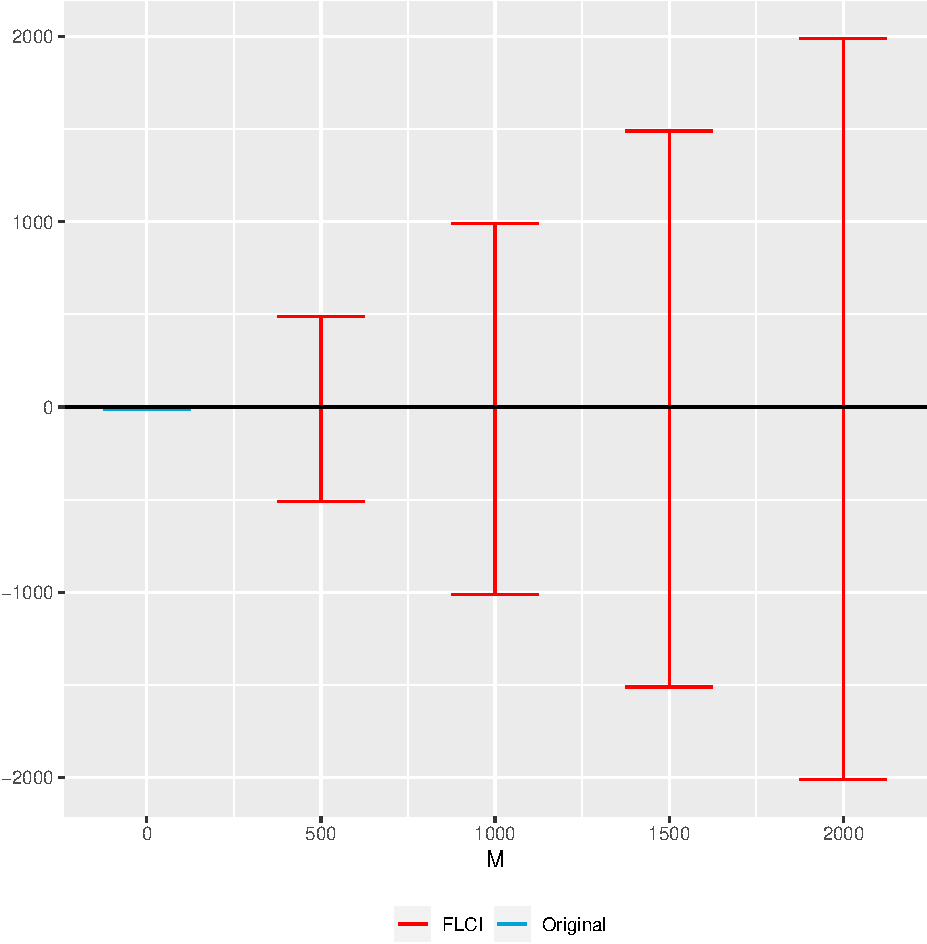
\includegraphics[width=.49\linewidth]{Report_files/figure-latex/Fig-6-1} }\subfloat[Relative Magnitude\label{fig:Fig-6-2}]{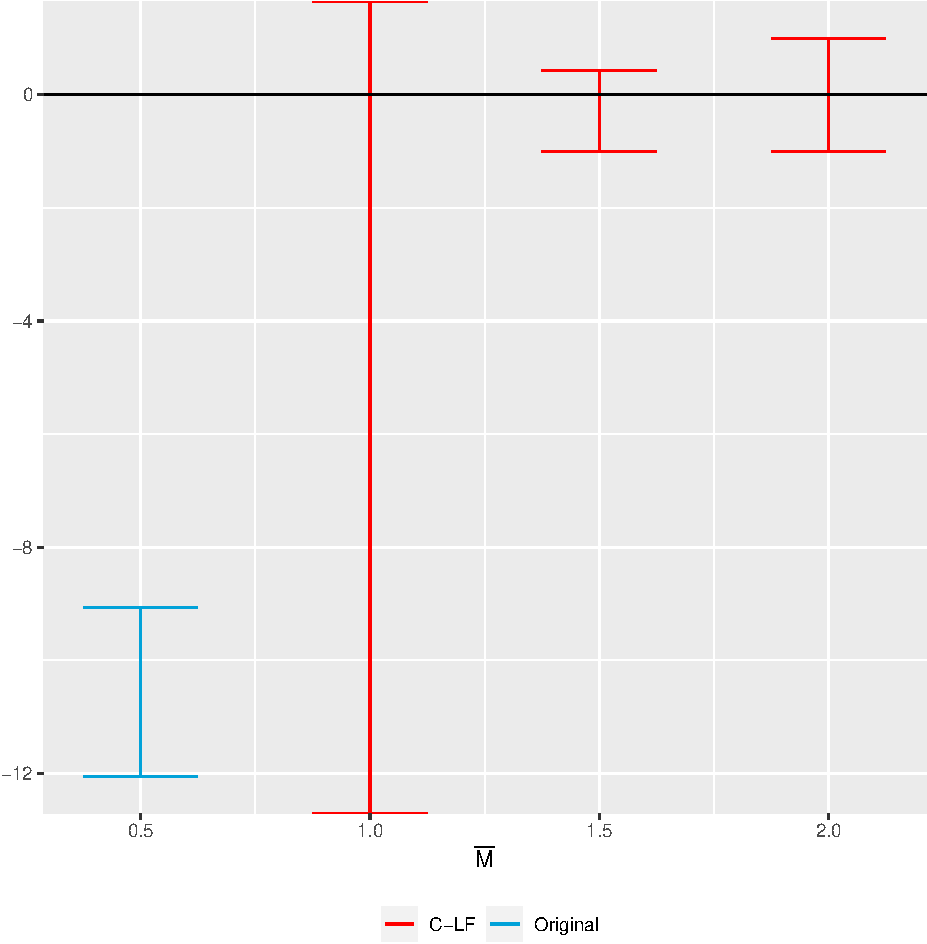
\includegraphics[width=.49\linewidth]{Report_files/figure-latex/Fig-6-2} }\caption{Rambachan and Roth (RR) Specification}\label{fig:Fig-6}
\end{figure}

\newpage

\hypertarget{discussion}{%
\section{Discussion}\label{discussion}}

Discuss your findings and compare estimates from different estimators
(e.g., are your results sensitive to different specifications or
estimators? Are your results sensitive to violation of parallel trends
assumptions?).

Across all different specifications we see a robust result, the ATE is
negative, that is the reduction in Uncomponsetad Care provided by
hospitals is due to the exogenous policy shock, the expansion Medicaid
across states. We have robust evidence to say this is a cusal effect.

\newpage

\hypertarget{reflection}{%
\section{Reflection}\label{reflection}}

Reflect on this assignment. What did you find most challenging? What did
you find most surprising?

The first challenge was to collect all data sets and merge them into
one, which requires a few programming skills and institutional knowledge
of the field. I encountered one specific problem while combining POS and
HCRIS data since I was not aware of the possibility that providers
changed the ownership compositions over time. I was not aware of this
situation until very late.

A second challenge was implementing the HonestDiD package. My results
were not interpretable or plausible when dealing with the original grid.

The main takeaways from this assignment is the importance of developing
a transparent and reproducible workflow that allows to make the changes
easily and improving my coding skills to avoid code repetition and
improve accuracy and efficiency.

\end{document}
